% Use only LaTeX2e, calling the article.cls class and 12-point type.

\documentclass[12pt]{article}

\usepackage{scicite}

\usepackage{times}

% Package for automaticall generating the table of contents

\usepackage[utf8]{inputenc}

% managing images
\usepackage{graphicx}
\graphicspath{ {images/} }
\usepackage{wrapfig}
\usepackage{amsmath}
\usepackage{blkarray}

\usepackage{setspace}
\onehalfspacing
\setlength{\parskip}{6pt}

\usepackage{physics}

\usepackage[margin=1in]{geometry}
\usepackage{sectsty}

\sectionfont{\fontsize{14}{17}\selectfont}
\subsectionfont{\fontsize{12}{15}\selectfont}

\pagenumbering{gobble}

\newenvironment{sciabstract}{%
\begin{quote} \bf}
{\end{quote}}

\title{An Introduction to Quantum Computing} 
\author
{Robert Olsthoorn\\
\\
\normalsize{University of Florida}\\
\normalsize{PHY3101: Modern Physics}\\
\normalsize{Fall 2015}\\
}

% Include the date command, but leave its argument blank.

\date{}



%%%%%%%%%%%%%%%%% END OF PREAMBLE %%%%%%%%%%%%%%%%

\begin{document} 



% Double-space the manuscript.

% Make the title.

\begin{figure}
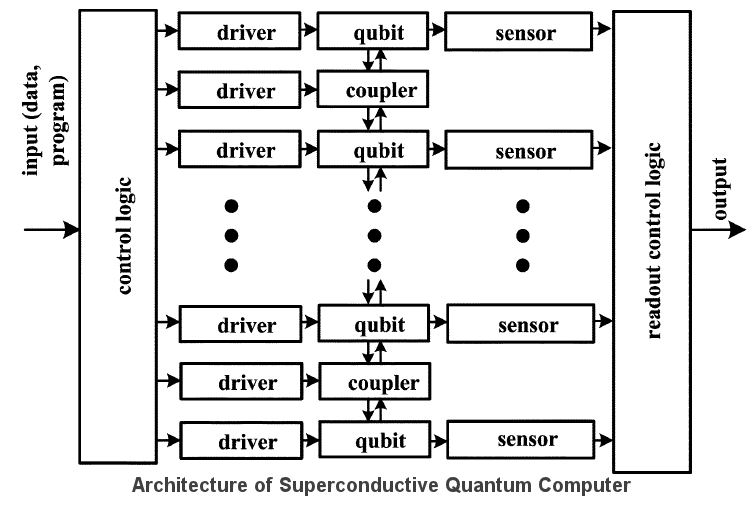
\includegraphics[scale=.5]{superconductive}
\centering
\end{figure}

\maketitle 

% Place your abstract within the special {sciabstract} environment.

\newpage

\begin{sciabstract}
\section*{Abstract}
Quantum computing is a potentially revolutionary principle which will be continued to be researched and studied for the foreseeable future as the importance of efficiency and the limit of binary computing is approached. This paper aims to provide an overview of the field of quantum computing for individuals with a minor understanding of physics, computer science, and mathematics. An introduction to quantum computing will leave the reader with a comfortable overview of the field and insight into which topic in particular they find most interesting.\par
This paper will talk briefly about the recent history of quantum computing as well as a small subset of quantum mechanicss as it relates to quantum computations and the cornerstones which currently make quantum computing possible. It aims to establish the differences between conventional and quantum computing with a goal to speak about how certain algorithms will run more efficiently and what applications in the field this can be used for. Near the end, we will look at the current issues within the field and its future importance.

\end{sciabstract}

\newpage

\tableofcontents

\newpage
\pagenumbering{arabic}

\section{History}

Quantum computing is a relatively new field in relation to computer science as a discipline with the informal start originating in the late 1970's and early 1980's as Richard Feynman speculated that quantum mechanics could not be effectively modeled through a classical computer. In accordance with Moore's law, the size of a silicon ship would continue to shrink until the individual elements were no larger than several atoms and would be subject to quantum effects at that scale. Feynman published an abstract model in 1982 in which he analyzed the outcome of using a quantum simulator in order to avoid the exponential slowdown which is common with classical computers.\cite{web}\par
In 1985, David Deutsch published a paper proving that any physical process could be, in theory, effectively rendered on a quantum computer. As a result, a quantum computer, which is able to operate in an exponential time, could provide a wide array of values for heavy data crunching, modelling of complex systems, or in the general solving NP-Complete classical problems in polynomial time.
\footnote{In computational complexity theory, a decision problem is NP-complete when it is both in NP and NP-hard. The set of NP-complete problems is often denoted by NP-C or NPC. The abbreviation NP refers to ``nondeterministic polynomial time''.\\Although any given solution to an NP-complete problem can be verified quickly (in polynomial time), there is no known efficient way to locate a solution in the first place.}
Deutsch proved a basic algorithm which will be worked through later in the paper. \par
Until 1994, the quantum computing field remained relatively unchanged until Shor was able to prove and set a method for a common NP-Hard factorization problem which could call on the benefits allowed through quantum computers, which would run in a time much shorter than what will be ever possible on classical computers.\cite{web} As a field, this momentus finding was able to push the field of research for quantum computing out of the view of the select who were performing research on the project to the public eye. Shor's algorithm will be explored later in the paper as well.\par

\section{Quantum Concepts and Theories}

As a quick note, the material that will only be covered consists of a very small section of quantum mechanics encompassing finite dimenstional quantum mechanic where the vector spaces which represent the states of the dimension are finite in size.\par

\subsection{Double Slit Experiment}
Young's double slit experiment is one of the most foundational experiments related to the field of quantum mechanics and demonstrates the wave-particle duality of photons when conducted. Before approaching the quantum model, it is interesting to explore a classical model and the probabilities associated with it before moving on.\par
\begin{wrapfigure}{L}{0.5\textwidth}
  \centering
  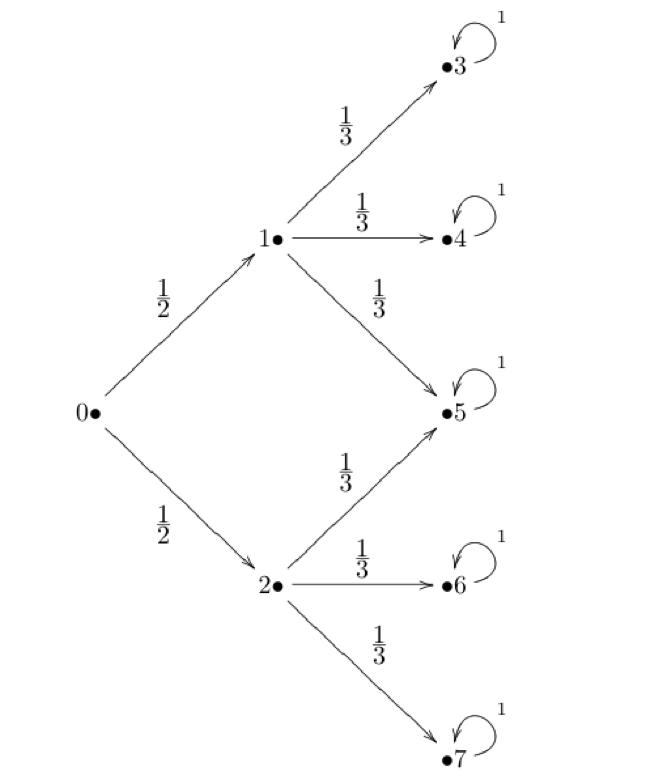
\includegraphics[width=0.5\textwidth]{classicslit}
  \caption{Corresponding graph to scenario}
\end{wrapfigure}
Pretend for a moment, that there is an experiment where there is a sharpshooter who is guaranteed to always shoot through one or the other open windows, with equal probability. Once the bullet passes through the window, it has an equal probability of hitting three targets. There is one target which is shared between both open windows.\par
The probability matrix associated with this scene is shown. 
\begin{figure}
  \centering
  \caption{Matrix representing the progression after one time click}
  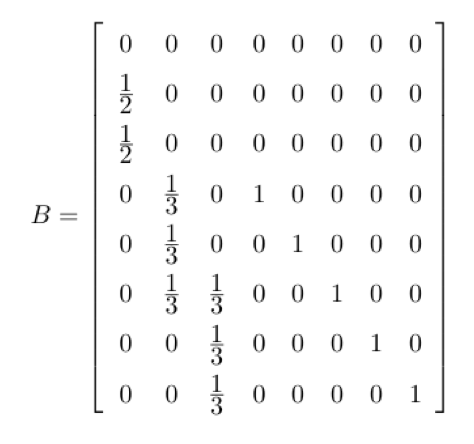
\includegraphics{classicB}
\end{figure}
\par
By representing the data points as a matrix, it is possible to identify the probability where the bullet might be found on the next time click by simply using matrix multiplication.\cite{intro}. The matrix shown above, \textit{B}, represents the state of the system after one time click. By multiplying the matrix by itself you are able to represent the state after two time clicks. 
\begin{figure}
  \centering
  \caption{Matrix representing the progression of two time clicks}
  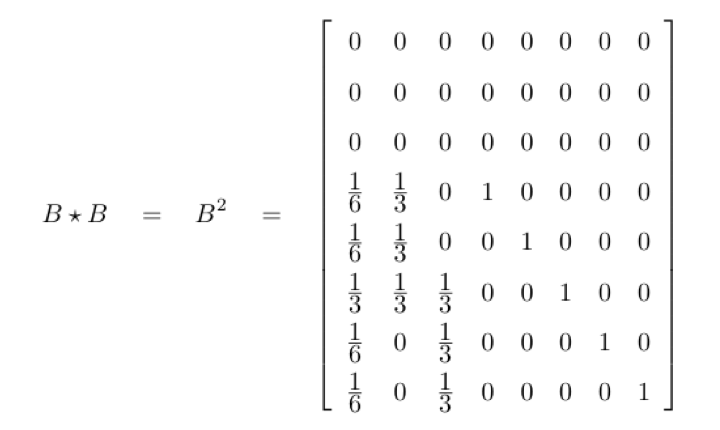
\includegraphics[width=0.5\textwidth]{classicB2}
\end{figure}\par
The takeaway from this example is to show that after two time clicks the bullets will be in the state \[B^2X = [0,0,0,\frac{1}{6},\frac{1}{6},\frac{1}{3},\frac{1}{6},\frac{1}{6}]^T\]
Which means that \(B^2[5,0]\) is equivalent to \(\frac{1}{3}\). Which is the two states \(\frac{1}{6}+\frac{1}{6}\).\par

\begin{wrapfigure}{L}{0.5\textwidth}
    \centering
    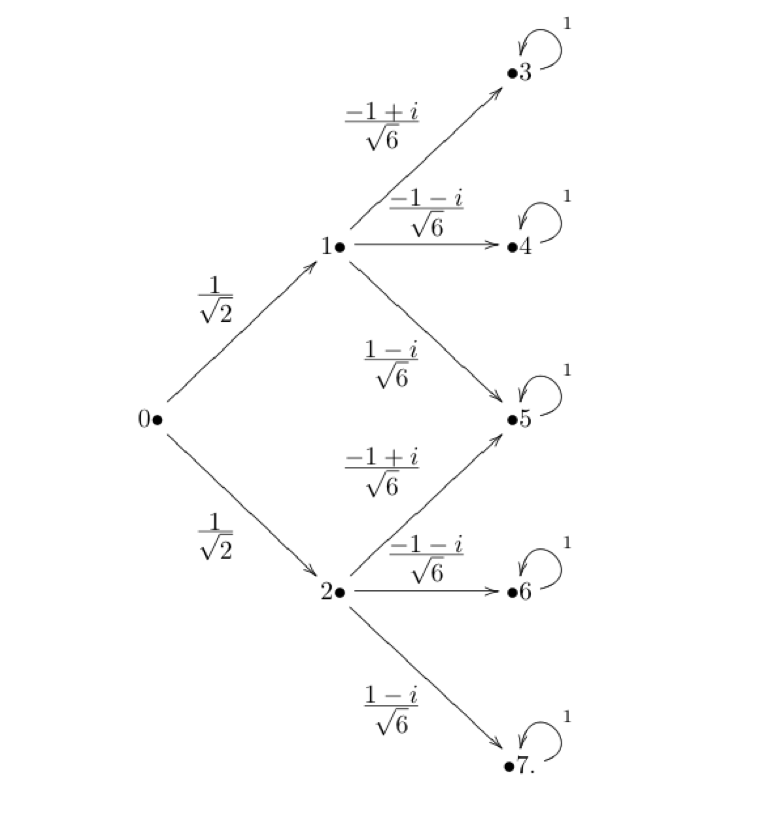
\includegraphics[width=0.5\textwidth]{quantumslit}
    \caption{Corresponding quantum modulus graph to scenario}
\end{wrapfigure}
Pretend for a moment that the shooter has now been changed to a flashlight which can spread light into both of the windows with a similar setting. Once the light has passed through the windows, it again travels randomly to one of the three respective target locations. Represented in this graph is the modulus, where the modulus squared represents the probabibility of the specific event taking place. $\frac{1}{\sqrt{2}}^2$ is $\frac{1}{2}$ and more importantly $\left|\frac{\pm 1 \pm i }{\sqrt{6}}\right|^2 = \frac{1}{3}$  \footnote{The complex number weights represented here are not to represent the actual quantum probability weights as this would require acquiring the distance of the slit spacing, the width of the individual slits. Rather the numbers given are to represent the point of quantum interference which will be highlighted later on}
\begin{figure}
	\centering
	\caption{Matrix representing the state after one time click}
	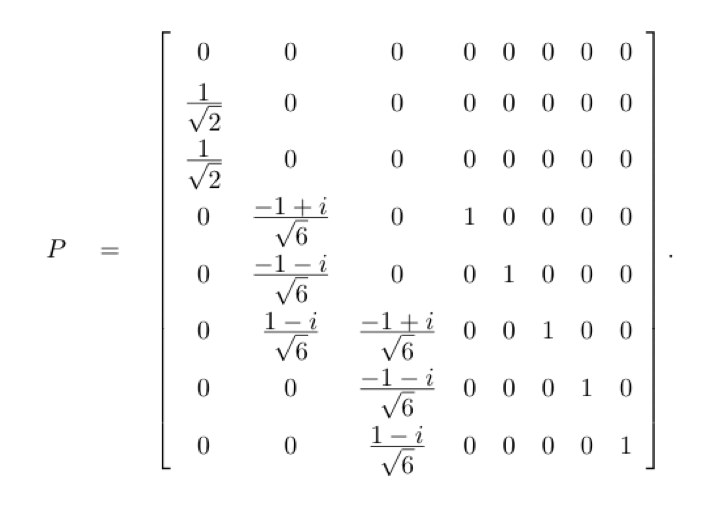
\includegraphics[width=.5\textwidth]{quantumP}
\end{figure}
\begin{figure}
	\centering
	\caption{Matrix representing the state after two time clicks}
	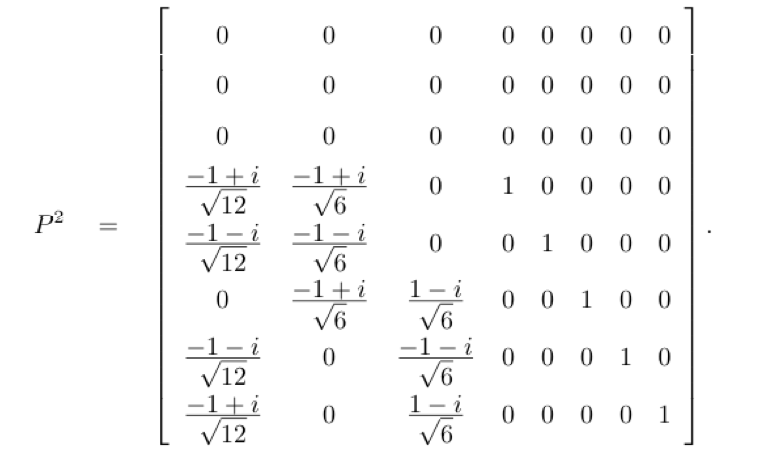
\includegraphics[width=.5\textwidth]{quantumP2}
\end{figure}
The above matrices represented the state of the experiment using the moduli of the components. In order to interpret this information in reference to the classical scenario it is helpful to consider the probability of the individual locations. This can be shown by squaring the individual components of the $P^2$ matrix.
\begin{figure}
	\centering
	\caption{Probability matrix of the modulus squared after two time clicks}
	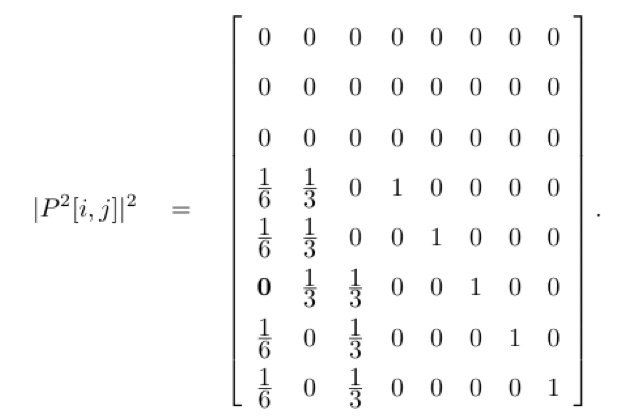
\includegraphics[width=.5\textwidth]{quantumProbability}
\end{figure}
\par
For the most part, the probability matrix for $P^2$ is the same as the probability matrix for $B^2$; however, there is one important distinction to be made. Which is that while $B^2[5,0] = \frac{1}{3}$ in the quantum simulation $P^2[5,0] = 0$. On a mathematical basis, this is trivially written as 
$$\frac{1}{\sqrt{2}}\bigg(\frac{-1+i}{\sqrt{6}}\bigg) + \frac{1}{\sqrt{2}}\bigg(\frac{1-i}{\sqrt{6}}\bigg) = \frac{-1+i}{\sqrt{12}} + \frac{1-i}{\sqrt{12}} = 0$$
This may seem troubling at first, but it must be remembered that photons are subject to particle interference and thus, on the shared target of the windows, the probability drops to 0. Furthermore, one may try to argue that if the experiment was carried out using only one photon, then the probability would again return to $\frac{1}{3}$, but this assumption would also be incorrect. A single photon is said to have a superposition in being in every possible position simultaneously. This is not mimicked in the classical world; however, due to the photon residing in every position at once it is prone to interference when the shared target is reached. As with most quantum phenomena, the particle is only determined to be in a certain state with a certain probability when a measurement is taken. In quantum mechanics, a measurement causes the superposition state to collapse to a certain pure state.\cite{intro}\par
This phenomena is central to the success of quantum computing, as it allows for an exponential number of comutations or simulations to be run in parallel thus becoming exponentially more efficient.

\subsection{Unitary Transformations}
The complex numbers which represent the quantum position are commonly known as the amplitudes of the wave function. A core theory in regards to quantum systems is the idea of a unitary transformation. Provided that the entire amplitude function $\Psi$ can be identified through a vector, a unitary transforamtion is a multiplication of those vectors by a transformation matrix whose inverse equals its conjugate transpose. \cite{cis4930}
The inherent properties of unitary transformations indicate that the total probability of the set always remains the same where the sum of the squares of the amplitudes is equivalent to 1 and that all changes are preserve the information across all states. Once a quantum state is observed in an isolated system, the quantum state is determined for all past and future times.\par
Furthermore, unitary transformations are fully reversible. This property can be shown to be true because $\ket{\psi} \mapsto U\ket{psi}$ preserves the normal standardization across states it can then be set that $1 = \bra{\psi}\ket{\psi} = \bra{\psi}U^ \dagger U\ket{\psi} $ for all unit vectors $\ket{\psi}$. By linearity it follows that $U^\dagger U = I$ which indicates invertibility. 
\footnote{The format used is known as bracket notation and will be understood in the following subsection. Where the $\bra{x}$ represents the ``bra'' section and the $\ket{x}$ represents the ``ket'' section and the entire representation can be shown by $\bra{x}\ket{x}$}

\subsection{Bracket Notation}
An $n$ dimensional quantum system indicates that a particle can be in one of $n$ states or positions. The quantum system could also represent the energy level of the photon polarization direction; however, for the purpose of defining the bracket notation consider just the position of the particle.\footnote{This section focuses on the ``ket'' of the bracket notation. The matching ``bra'' $\bra{x}$ denotes the conjugate transpose of $\ket{x}$. This choice is arbitrary, but is the convention which is widely used when talking about quantum computing \cite{non}}\par
The state $$\ket{\psi} = [0,1,0,0,...,0]^T$$ is to represent that the particle is found at position 1. Similarly the state $$\ket{\psi'} = [0,...,1,...,0]^T$$ is said to be found at the position $j$ where the particle can be found. These states, where the particle can be certainly found are known as pure states. A superposition of the general form $$\ket{\phi} = [c_0, c_1,...,c_{j},...,c_{n-1}]^T$$ can be added to another superposition state simply by adding elements individually. Adding the inital to $$\ket{\phi'} = [c_0', c_1',...,c_{j}',...,c'_{n-1}]^T$$ yields
$$\ket{\phi} + \ket{\phi'} = [c_0+c_0', c_1+c_1', ..., c_{j}+c'_{j},..., c_{n-1} + c'_{n-1}]^T$$ This process of adding the complex vector spaces are valid and yied accurate results.\par
The only component which matters is not the length $\ket{\phi}$, but the direction of the component. Working with these vectors, it makes more sense to work with a normalized version of the vector $$\frac{\ket{\phi}}{\left|\ket{\phi}\right|}$$\par

While this works for adding the superposition states together in order to combine quantum systems it becomes necessary to calculate the tensor product \footnote{SOME INFORMATION ON THE TENSOR PRODUCT PLACED IN HERE}. If we take $\ket{\phi}$ to be the first quantum system and take $\ket{\phi'}$ to be the second quantum system we represent the combined system as $$\ket{\phi}\otimes\ket{\phi'} = \ket{\phi, \phi'} = \ket{\phi \phi'}$$

\subsection{Observations}
As mentioned before, when a quantum superpositiion state it condenses to a single pure state in order for the experiment to show the particle at a single position. In an attempt to predict which state the particle will condense to we look at the sum of the squares of the modulus\cite{intro} 
$$S = \left|c_0\right|^2 + \left|c_1\right|^2 + \left|c_{j}\right|^2 +\left|c_{n-1}\right|^2$$ 
Therefore there is a $\left|c_0\right|^2\!/S$ chance of the superposition collapsing to the $0th$ pure state and a $\left|c_1\right|^2\!/S$ chance of collapsing to the $1st$ pure state as the way that the quantum state collapses is random, but can be represented as a hermitian.
\footnote{an $ n\times n $ matrix is considered hermition if $A = A^\dagger $. In other words, only if $ A^T = \overline{A} $}
\par
\textbf{Eigenvalue} is a real number which can be found in a hermitian matrix if for a matrix $A$ in $M^{n\times ns}$, there is a number $m$ in $M$ and a vector $\ket{\phi}$ in $M^n$ such that $A\ket{\phi} = m\ket{\phi}$. $m$ in this case is an Eigenvalue, where $\ket{\phi}$ is known as a \textbf{Eigenvector} of $A$ associated with $m$.\par
All eigenvalues in a hermitian matrix are all real numbers. Furthermore, distinct eigenvectors which have distinct eigenvalues of a hermitian matrix are orthogonal. It follows that the set of eigenvectors form a basis for the entire complex vector space which represents the quantum of interest. \cite{intro}. Taking $A\ket{\phi} = m\ket{\phi}$, it becomes obvious that, as stated before, the only part of the state that matters is the direction rather than the length. This means that $m\ket{\phi} = \ket{\phi}$ A critical assumption which can be made following this statement is that if the current state of the quantum system is based on the eigenvector basis, than the system will not change.
\section{Qubit}
Fundamentally, a bit is the state of any system. A classical bit represents one of two distinct positions for a scenario as in a 1 or 0, on or off, true or false. In classical computers all data is stored, shuttled, and interpreted through 1's or 0's. Due to the binary state of data, this limits the number of computations that can be done at any single time on a classical machine.\par
Quantum bits (qubits), rather, is a unit vector in a two dimensional complex vector space. When observed a quantum bit will settle into either a $\ket{0}$ or $\ket{1}$ binary state. The implementation of a qubit could correspond to the polarization of the photon or the spin-up or spin-down components of an electron.\cite{non} A quantum bit can be represented as a superposition of $\ket{0}$ or $\ket{1}$ such that $a\ket{0}+b\ket{1}$ where $a$ and $b$ are complex numbers such that $\left| a\right |^2+\left| b\right| ^2 = 1$.\par
An important consideration is that the state can only be measured once. Though it may seem possible to clone a qubit so that it may be measured in two possible ways, this is impossible. Because quantum states are subject only to unitary transformations, cloning is not allowed. The proof, established in 1982 by Wooters and Zurek, is an example of the linearity of unitary transformations.\cite{non}\par
Assume that $U$ is a unitary transformation which is possible to clone so that in all quantum states $\ket{a}, U(\ket{a0}) = \ket{aa}$. Let $\ket{a}$ and $\ket{b}$ be orthogonal quantum states. And $U(\ket{a0}) = \ket{aa}$ and $U(\ket{b0}) = \ket{bb}$. Consider the case $\ket{c} = (1/\sqrt{2})(\ket{a} + \ket{b})$.
\begin{align*}
U(\ket{c0} &= \frac{1}{\sqrt{2}}(U(\ket{a0})+U(\ket{b0}))\\
&= \frac{1}{\sqrt{2}}(\ket{aa}+\ket{bb})
\end{align*}
But since U was defined as a cloning transformation
\begin{align*}
U(\ket{c0}) &= \ket{cc}\\
&= (\frac{1}{\sqrt{2}}(\ket{aa}+\ket{bb}))^2\\
&= \frac{1}{2}(\ket{aa}+\ket{ab}+\ket{ba}+\ket{bb})
\end{align*}
which is not equal to $(1/\sqrt{2})(\ket{aa}+\ket{bb})$. This proves that there is no unitary operation to clone unknown quantum states. This \textit{no cloning} principle is only valid for unknown quantum states, as it is in fact possible to clone known quantum states. Though it is possible to obtain particles in an entangled state from an unknown state.

\subsection{Notation}
The notation for qubits which will be used follows the format as a two by one matrix with complex numbers.
$$ 
\begin{blockarray}{cc}
\begin{block}{c[c]}
0 & c_0 \\
1 & c_1 \\
\end{block}
\end{blockarray}
$$

where $\left| c_0\right |^2 + \left| c_1\right |^2 = 1$. In order to get a better idea of the qubit take the vector
$$ V = 
\begin{blockarray}{c}
\begin{block}{[c]}
5 + 3i \\
6i \\
\end{block}
\end{blockarray}
$$
and find the magnitude so that it may be normalized
$$ \left| V \right| = \sqrt{\langle V, V \rangle} = \sqrt{
  [5-3i, -6i]
\begin{blockarray}{c}
\begin{block}{[c]}
5 + 3i \\
6i \\
\end{block}
\end{blockarray}
} = \sqrt{34+36} = \sqrt{70}
$$
therefore
$$ \frac{V}{\sqrt{70}} = 
\begin{blockarray}{c}
\begin{block}{[c]}
\frac{5 + 3i}{\sqrt{70}} \\
\frac{6i}{\sqrt{70}} \\
\end{block}
\end{blockarray}
$$
Now that the vector has been normalized, we can obtain the probabilities of each individual scenario and the probability of being in state $\ket{0}$ is $34/70$ while probability of state $\ket{1}$. TODO CHANGE ALL THE NUMBERS IN HERE TO BE DISTINCT FROM THE ONES BEFORE\par
For one qubit, it is easy to normalize and find the values, but in order to extract any real value from quantum computing it would serve well to consider a state with several qubits in progression. A typical byte of computer information contains 8 bits and might look like the following $$ 11110010 $$ which in unsigned binary would represent the number $242$. Using a classical bit, the number of possible results is $2^8 = 256$.\par
As a set of qubits, we can represent this number by a sum of the tensor products. 
$$ \ket{1}\otimes\ket{1}\otimes\ket{1}\otimes\ket{1}\otimes\ket{0}\otimes\ket{0}\otimes\ket{1}\otimes\ket{0}\otimes $$
To represent the above values of the quantum bits in a matrix 
$$ 
\begin{blockarray}{cc}
\begin{block}{c[c]}
00000000 & c_0 \\
00000001 & c_1 \\
\vdots & \vdots \\
11110001 & c_{241} \\
11110010 & c_{242} \\ 
11110011 & c_{243} \\ 
\vdots & \vdots \\
11111110 & c_{254} \\
11111111 & c_{255} \\
\end{block}
\end{blockarray}
$$
where each of the 256 qubytes holds 8 qubits. A state of 8 qubits is given by writing 256 complex numbers. In order to store the $2^{64}$ qubits you would need to have a memory storage size equivalent to $\approx 2.3$ exabytes. This is an amount of data which vastly outweighs the amount of digital data currently handled by any individual company. \cite{storage}
\subsection{Implementation}
FILL THIS OUT IF YOU NEED MORE INFORMATION ON IMPLEMENTATION
\subsection{Quantum Gates}
In order to use classical bits to do any valuable solving, logic gates need to be implemented in order to change output based on the state of the inputs. For classic bits, there are common AND, OR, and NOT operators, for quantum bits there are equivalent gates known a quantum gates which because of linearity the transformations can be exemplified by their effect on the basis vectors. These transformations can easily be proven to be unitary.
$$
Identity\:Matrix: 
\begin{blockarray}{cc}
\begin{block}{(cc)}
1 & 0\\
0 & 1\\
\end{block}
\end{blockarray}
 \:causes\:
\begin{blockarray}{c}
\begin{block}{[c]}
0\\
1\\
\end{block}
\end{blockarray}
\rightarrow
\begin{blockarray}{c}
\begin{block}{[c]}
0\\
1\\
\end{block}
\end{blockarray}
\\
$$

$$
Negation\:Matrix: 
\begin{blockarray}{cc}
\begin{block}{(cc)}
0 & 1\\
1 & 0\\
\end{block}
\end{blockarray}
 \:causes\:
\begin{blockarray}{c}
\begin{block}{[c]}
0\\
1\\
\end{block}
\end{blockarray}
\rightarrow
\begin{blockarray}{c}
\begin{block}{[c]}
1\\
0\\
\end{block}
\end{blockarray}
$$

$$
Phase\:Shift\:Matrix: 
\begin{blockarray}{cc}
\begin{block}{(cc)}
1 & 0\\
0 & -1\\
\end{block}
\end{blockarray}
 \:causes\:
\begin{blockarray}{c}
\begin{block}{[c]}
0\\
1\\
\end{block}
\end{blockarray}
\rightarrow
\begin{blockarray}{c}
\begin{block}{[c]}
0\\
-1\\
\end{block}
\end{blockarray}
$$
These matrix shifts are the building blocks of most quantum gates. A basic NOT gate is instrumental to the success of any algorithm which will be used. The controlled-NOT gate $C_{not}$ operates on two qubits by changing the second bit if the first bit is one and not changing it if the first bit is 0. Though there are various forms that the $C_{not}$ gate could be written, one is displayed below.
$$
C_{not}\:Matrix: 
\begin{blockarray}{cccc}
\begin{block}{(cccc)}
1 & 0 & 0 & 0\\
0 & 1 & 0 & 0\\
0 & 0 & 0 & 1\\
0 & 0 & 1 & 0\\
\end{block}
\end{blockarray}
 \:causes\:
\begin{blockarray}{cc}
\begin{block}{[cc]}
0 & 0\\
0 & 1\\
1 & 0\\
1 & 1\\
\end{block}
\end{blockarray}
\rightarrow
\begin{blockarray}{cc}
\begin{block}{[cc]}
0 & 0\\
0 & 1\\
1 & 1\\
1 & 0\\
\end{block}
\end{blockarray}
$$
The transformation $C_{not}$ is unitary since $C^*_{not} = C_{not}$ and $C_{not}C_{not} = I$ where $I$ is the identity matrix. the $C_{not}$ gate is not able to be decomposed into two single bit transformations.\cite{non}\par
\section{Applications}
Though quantum computing is still a relatively young field, it has been propelled out of the view of just the researchers who were pursuing it as an interesting exploration of quantum mechanics into the field of high performance computing thanks primarily to the applications which have already been discovered and the potential applications that could be found in the near future. Currently, quantum computing is being explored within the realm of database searching using Grover's algorithm, which searches over an unsorted set of data in $\sqrt{n}$ time rather thean $n$ time. Also, quantum computing would allow for more effective modeling of quantum mechanics systems which are currently very resource intensive. In addition, it could prove valuable for modelling proteins and molecules and potentially simulating many different unique scnearios in this regard in order to discover solutions to existing medical problems. However, because the field is young, many implementations on a large scale are yet to be seen, and are still to be proven.
\subsection{Current Implementation}
There are a number of proposals in order to actually build a quantum computer using ion traps, nuclear magnetic resonanace, optical and solid state techniques. \cite{non} However, all of these proposed implementations come with their own set of flaws and are mostly limited by the scale at which they can operate.
\subsection{Encryption}
Classically, in order to communicate in a secure manner between two people, public key encryption is used which relies on the multiplication of two large prime numbers to obtain a key, commonly known as RSA encryption.\par 
\begin{wrapfigure}{R}{0.5\textwidth}
    \centering
    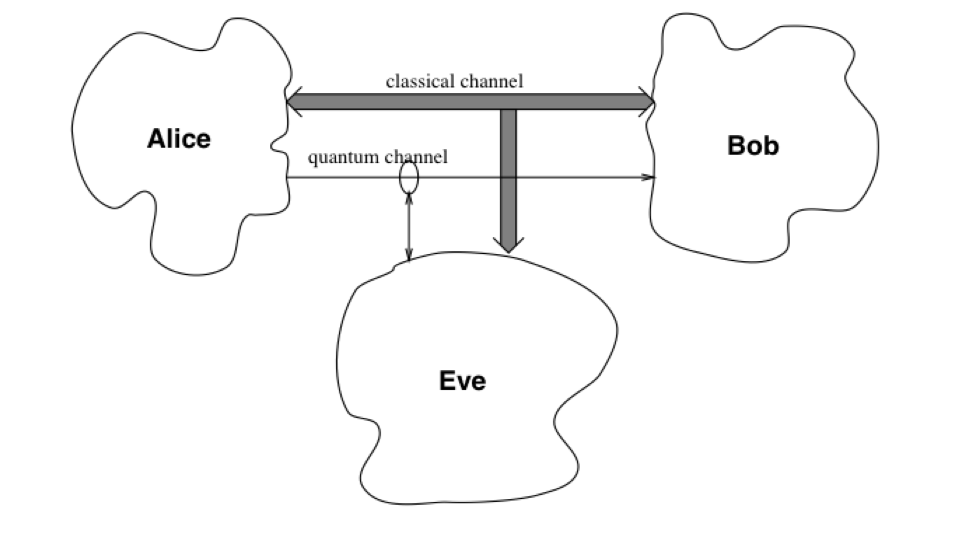
\includegraphics[width=0.6\textwidth]{alice}
    \caption{Alice and Bob graphic}
\end{wrapfigure}
Alice and Bob, are attempting to agree on a secret key so that they may communicate in private; however, a third person Eve, has access to their two channels of communication. The first channel is bi-directional for sending messages while the second channel is uni-directional with a transfer limit of only sending individual particles at once for establishing which key should be used. To establish the private key, Alice sends bits to Bob after encoding them in the quantum state of a photon. Alice randomly chooses one of two bases for encoding each bit.\footnote{The notation used below indicates the direction in which the photon is polarized. Depending on the direction of the polarization, photons will be measured with varying levels of success. Note that $\ket{\rightarrow} = (1/\sqrt{2})(\ket{\nearrow}-\ket{\nwarrow})$ and $\ket{\uparrow} = (1/\sqrt{2})(\ket{\nwarrow}+\ket{\nearrow})$. Thus photons passing through $A$ with state $\ket{\rightarrow} $ will be measured by $B$ as $\ket{\nearrow}$ with probability $.5$.\cite{non}}
\begin{align*}
&0\rightarrow \ket{\uparrow}\\
&1\rightarrow \ket{\rightarrow}\\
\end{align*}or\begin{align*}
&0\rightarrow \ket{\nearrow}\\
&1\rightarrow \ket{\nwarrow}\\
\end{align*}
Bob randomly picks a basis to use, and at the end of the message stream communicates that choice to Alice. With this knowledge, they can determine which bits have successfully transferred and can use these bits as the key. They will discard about 50\% of data.\par
If Eve were to measure the state of the photons, she would have to randomly pick a basis to use when resending it resulting in a wrong basis selected 50\% of the time. This will lead to Bob to read the wrong value 25\% of the time. A higher error rate will be found, and thus detected so that Alice and Bob are aware that a thrd party (Eve) is listening in.
Though many different techniques for creating quantum keys have been explored, none are substitutes for classic public key encryption systems.
\subsubsection{Cracking public key}
Uses shor's algorithm
\subsection{Algorithms}
Due to the exponential factor of the amount of states qubits can be in, an algorithm can be made to speed up the run time of NP-Hard and NP-Complete problems to run in closer to polynomial time. One example of this is prime factorization which is solved by Shor's algorithm and search on an unordered set which is solved by Grover's algorithm.
\subsubsection{Shor's Algorithm}
Shor's algorithm is of particular importance to certain government agencies, because current attempts at factoring of public keys would take years on a clasical computer. Factoring a number in polynomial time relies on being able to find the order\footnote{The ``order'' concept is TODO FILL IN INFORMATION HERE} of a number mod $N$.\cite{cis4930} Provided that this can be found then the algorithm is as follows
\begin{enumerate}
\item Pick a random $x<N$
\item Compute $f = $gcd$(x, n)$; if $f\neq 1$, return $f$ (As it is a factor)
\item Find the least $r$ such that $x^r\equiv 1 ($mod$\:N)$ (Where r is the repetition period)
\item If either gcd$(x^{r/2}-1, N)$ or gcd$(x^{r/2}+1, N)$ is not 1, return it, as a factor
\item Else, repeat from step 1
\end{enumerate}
The number of repetitions that this loop requires is run in polynomial time if every step can be run in polynomial time. Upon analysing the steps, step 3 where $x^r$ must be computed is necessary. In order to solve this, Shor used an application of the fourier transform which relies on quantum parallelism. The mathematics behind this approach falls beyond the scope of this paper
\footnote{The quantum fourier transform is linear transformation on quantum bits, and is the quantum analogue of the discrete Fourier transform. The quantum fourier transform is in fact a unitary operation as required by operations done on a quantum machine}; however, it is assumed that it is a valid approach. The algorithm is as follows. The machine computes all of $x^r$ for all $r<N^2$ simultaneously. The series, $x^r(($mod $N))$ repeats in cycles if $x4$ is relatively prime to $N$. This cycle is stored in $N^2$ distinct states which corresponds to the $N^2$ different values. The quantum fourier transform is now appplied to the superposition of the resulting states and the algorithm ecnodes the frequency spectra for finding different values of $x^r$ mode $N$. The amplitude peaks found will correspond to multiples of the basic repetition period of $x^r$. By measuring the state, we will attain with a high probability the value of the repetitive state needed. This process runs in polynomial time. \cite{cis4930}
\subsubsection{Grover's Algorithm}
Grover's algorithm is of particular importance to any large technology-based company which has a data stored in a database where some liens of data need to be found by searching through the article. This process of searching is also incredibly relevant in sorting algorithms, as most sorting algorithms rely on finding either a smaller or larger number for the comparison based sorting algorithm to functino properly. While this is valuable, most databases are already sorted in regards to a particular context, so Grover's search algorithm operating within the scope of a heuristic algorithm\footnote{A heuristic algorithm simply means that the algorithm has an idea before computation of what the data might look like and so can make an assumption which should perform favorably.} has shown that a quadratic speed-up is possible when compared to a classical heuristic.\cite{non}\par
Grover's algorithm follows the steps outlined below:
\begin{enumerate}
\item Prepare a register containing a superposition of all possible values $x_i \in [0,1,...,2^n-1]$.
\item Compute $P(x_i)$ on this register where the superposition is calculated $$\frac{1}{\sqrt{2^n}}\sum^{n-1}_{x=0}\ket{x, P(x)}$$
\item Change amplitude of $a_j$ to $-a_j$ for $x_j$ such that $P(x_j) = 1$. Overall the amplitudes will now look like 
\begin{figure}[hb]
  \centering
  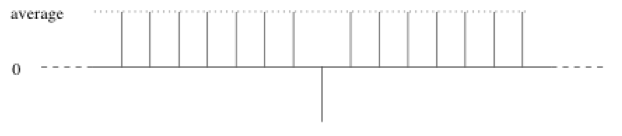
\includegraphics[width=.5\textwidth]{amplitude}
\end{figure}
\item Apply inversion about the average to increase amplitude of $x_j$ with $P(x_j)=1$
\begin{figure}[hb]
  \centering
  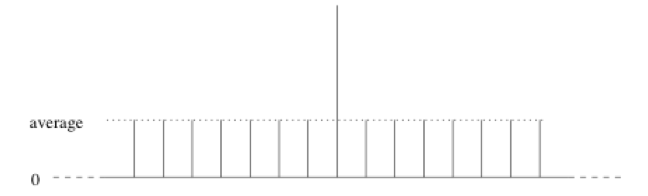
\includegraphics[width=.5\textwidth]{amplitude2}
\end{figure}
\item Repeat steps 2 through 4 $\frac{\pi}{4}\sqrt{2^n}\:$ \footnote{This number is to ensure that the execution stops when the desired state is hit. This number could be proven by the fourier transform application by Brassard} times
\item Measure the end result

\end{enumerate}
An interesting observation is that while classical algorithms will get a more accurate solution if they repeat over and over again, a quantum algorithm will peak when it gets close to the desired state for a solution and becuase all the transformations are unitary it will move farther and farther away from the desired state. In order to obtain valuable data from a quantum algorithm, it becomes imperative to understand when to stop the process. An extension of Grover's algorithm using fourier transforms to identify the optimal number of iterations has been written which does not increase the overall algorithm complexity\footnote{Algorithm complexity is commonly referred to in Big-O notation where O($n$) indicates that an algorithm runs in linear time, O($n^2$) runs in quadratic time, and O($2^n$) runs in exponential time}\footnote{This method written by Brassard in 1998\cite{non}.}.
\section{Error Correction}
\textbf{Decoherence}, or the distortion of the quantum state due to interactions with the outside environment, is the greatet difficulty that needs to be overcome in order to effectively scale them for large scale use.\cite{non} Though attempts were made to isolate the outside environment by lowering the temperature to near absolute zero, the breakthrough in solving this problem ultimately arose through the invention of quantum error correction handling techniques. This allowed for logic within the computer to detect when an error had been made and to correctly return it to an error free state. Although error correction is computationally intensive, it remains a valuable tool as long as the error probabiliy per gate resides below a certain acccuracy threshold
\par
The process of quantum error correction is a dissipative process and so produces waste heat that must escape from the device into the environment. As the errors occur, they are stored in a set of ancilla bits\footnote{\textbf{Ancilla bits} are extra bits which have a secondary role in a logic circuit}. To reuse the ancilla bits, they must be flushed which releases entropy into the environment in the form of heat.\cite{pro} This error correction technology will prove a challenge for computer engineers in the future as they try and keep the temperature of the computer as cool as possible.\par
\section{Future of Quantum Computing}
Unfortunately, research in the field of quantum computing has been moving at an incredibly slow pace mostly due to the difficulty in avoiding errors in the process or trying to correct them in the process. Quantum computing will continue to influence the field of experimental physics by providing new kinds of measurements and experiments. Before quantum computing ever goes mainstream, it will have a place in high precision physics laboratories where the results of tests held will lead to greater and more accurate error correction schema.\cite{pro}\par
Quantum computing will see a stronger and greater push as we approach the classical computation limit of Moore's law. The current limits of quantum computing, predominantly arising from error correction and errors with fault-tolerant gates, once mitigated will allow for a wide development in high performance computing and will open up new fields of research for years to come. The impact which industrial and commercial quantum computing will have is immeasurable.

% Your references go at the end of the main text, and before the
% figures.  For this document we've used BibTeX, the .bib file
% scibib.bib, and the .bst file Science.bst.  The package scicite.sty
% was included to format the reference numbers according to *Science*
% style.


\bibliography{scibib}

\bibliographystyle{Science}

\newpage

\begin{thebibliography}{1}
\bibitem{pro} 
Preskill, John. ``Quantum Computing: Pro and Con.'' Diss. California Instute of Technology, 1996. Print. 
\bibitem{non}
Rieffel, Eleanor, and Wolfgang Polak. ``An Introduction to Quantum Computing for Non-Physicists.'' Diss. FX Palo Alto Laboratory, 2000. Print. 
\bibitem{web}
West, Jacob. ``The Quantum Computer.'' An Introduction to Quantum Computing. Rice University, 28 Apr. 2000. Web. 25 Oct. 2015. 
\bibitem{intro}
Yanofsky, Noson S. ``An Introduction to Quantum Computing.'' Diss. Department of Computer and Information Science, Brooklyn College, CUNY, 2007. Print. 
\bibitem{cis4930}
CIS4930 Textbooks
\bibitem{storage}
http://www.comparebusinessproducts.com/fyi/10-largest-databases-in-the-world
\end{thebibliography}

\clearpage

\end{document}




















